
\documentclass[runningheads]{llncs}
%
\usepackage{graphicx}
\begin{document}
%
\title{Tile Pattern KL-Divergence for
Analysing and Evolving Game Levels: a review of Simon & Vanessa 2019~\cite{ref_lncs1}}
\titlerunning{Tile Pattern KL-Divergence}
\author{Hao Zhang }
\institute{Adelaide University, Australia \\
\email{a1788848@student.adelaide.edu.au}}
%
\maketitle          % typeset the header of the contribution
%

%
%
%
\section{INTRODUCTION}
This is a review of the article "Tile Pattern KL-Divergence for Analysing and Evolving Game Levels" by Simon & Vanessa 2019~\cite{ref_lncs1}.

The topic of this article is really attractive that to design an evolutionary algorithm called ETPKLDiv to make a Mario level similar to the sample level (which is the existing level in Super Mario Bros). Then, the authors compared ETPKLDiv  to 3 existing algorithms to measure the advantages of this evolutionary algorithm.

This article completes five challenges:
\begin{enumerate}
  \item Given a sample level (for example, Mario 1-1), find a way to represent the level design. (See section 3.1)
  \item Find existing PCG approach to make Mario levels. (See section 3.2)
  \item Find a formula to measure the fitness of each solution. (See section 3.3)
  \item Design an evolutionary algorithm called Evolution with Tile Pattern KL-Divergence (ETPKLDiv) based on the fitness measurement. (See section 3.4)
  \item Compare the ETPKLDiv algorithm to the existing algorithms and measure the solution quality and speed. Find the advantage of ETPKLDiv.(See section 3.5)
\end{enumerate}

Then, I will discuss my suggestion on how to improve the algorithm on evaluating if the level is passable and some general rules in Mario Bros. (section 4). 

Finally, I will give feedback on this article (section 5). 
\section{BACKGROUND}
Super Mario Bros. is a platform game by Nintendo. In this game, players need to control the character Mario and travel through the Koopa Kingdom and save Princess Peach. If Mario fall cliffs or is hurt by enemies, he will lose a life and then back to the beginning of the level until run out of all the lives or pass the level.

Using AI to make a 'good' game level can be seen as a real challenge because of the following reasons:
\begin{itemize}
\item To save all the information in a level takes too much space and will be hard to calculate, so most of the time, we need to find a way to represent the level design.
\item Measuring fitness is hard because it is hard to find a mathematical formula to calculate if people 'like' this level.
\item People often have their preferences so Even experienced game designers have a hard time creating levels that everyone likes, let alone AI.
\end{itemize}



\section{REVIEW OF THE ARTICLE}
This part will explain in detail how the 5 challenges mentioned in INTRODUCTION ( section 1) were completed in the reviewed article.

\subsection{Generate Data From Sample Level}
 The approach to generate and store the sample level design is to split the level into 1x1 tiles. We can store the level into a matrix of Identities (see Fig.1) so that the store usage will be minimized.
 
 \begin{figure}
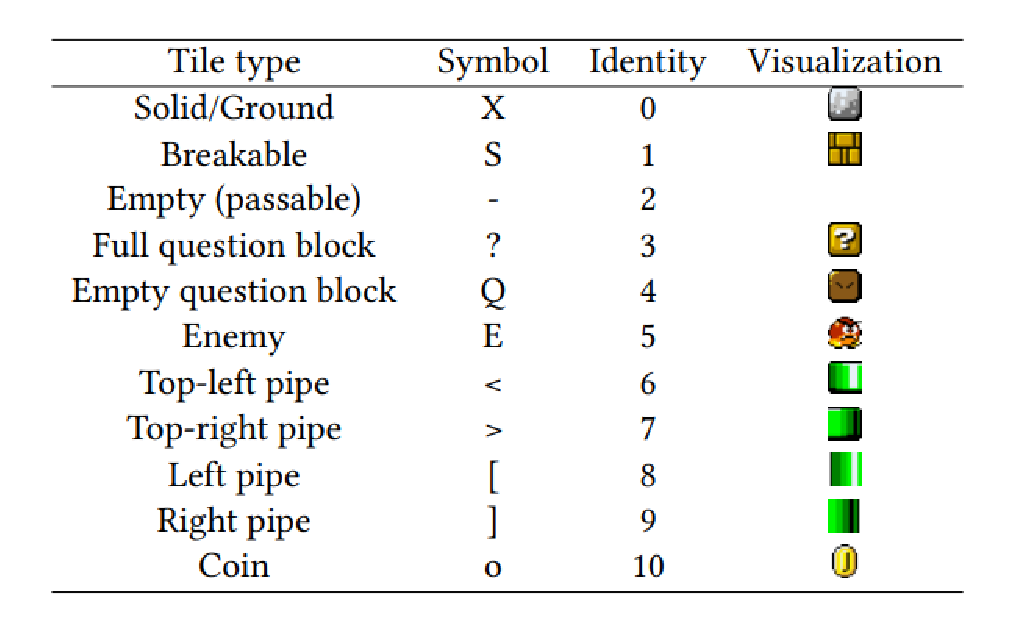
\includegraphics[width=0.5\textwidth]{Figure1.eps}
\centering
\caption{ ~\textbf{Tiles in Mario level and its representation.} The image presented is made up of symbol characters and integer identities that are translated to the relevant tile kinds in the Mario AI framework. This figure is  available in the research paper~\cite{ref_lncs1} on page 171.} \label{Figure1}
\end{figure}

\begin{figure}
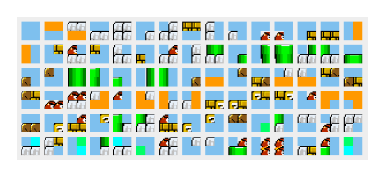
\includegraphics[width=0.5\textwidth]{Figure2.eps}
\centering
\caption{ ~\textbf{2*2 tile patterns generated from the sample level, shown from the most to least frequent} This figure is available in the research paper~\cite{ref_lncs1} on page 172.} \label{Figure2}
\end{figure}

To show the relationship between each tile in each sample level, the authors find a way that split the tile patterns into a size of N*N (for example, 2*2 or 4*4) so that every pattern contains the information of connecting tiles. Then based on the frequency of each pattern, make a probability distribution (see Fig.2).




\subsection{Existing PCG Approach To Make Mario Levels}
Based on search, the article's authors find 3 existing PCG approaches to make Mario levels.Those are WFC (Wave Function Collapse), GANs (Generative Adversarial Networks) and ELSGAN (Exploratory Latent Search GAN) which can also produce good result of Mario levels, which will be described below:

\subsubsection{Wave Function Collapse}
Wave Function Collapse (WFC) is a PCG approach that has recently been popular in designing game levels. This approach relies on putting patterns together to make it satisfy a way that a set of constraints is met (like a Sudoku game)~\cite{ref_article1}. 

For example, for generating a Mario level, one of the possible ways is: (1) Analyse the sample level and split all the tiles and record their neighbours (this is the constraints. When generating, all the tiles must have the neighbours they recorded, having new neighbours is not permitted). (2) Find a random place and fill in a random integer identity. (3) Find a place that is next to the existing tiles and has the minimized choices. (4) Fill this place with a possible choice randomly (but the possibility is influenced by the frequency). (5) Repeat steps 3 and 4 until all the place was full-filled (success) or constraints contradict (fail).

The description above is based on the article ~\cite{ref_lncs1} on page 172, section 2.2, but with personal understanding. This is a possible way to make Mario levels but may not be completely the same as the approach in the authors' experiments.

\subsubsection{Generative Adversarial Networks and  Exploratory Latent Search GAN}
Generative Adversarial Networks (GANs) and  Exploratory Latent Search GAN (ELSGAN) are also PCG approaches. ELSGAN is a further approach based on GAN by employing a latent vector search. The detail on how ELSGAN makes Mario levels is in here~\cite{ref_lncs2}.

The GANs and ELSGAN each have a generator and discriminator. The difference is that the generator in ELSGAN is a  multi-layer neural network, convert a vector [0,1] to real-valued vectors. And then use the real-valued vectors to make a new Mario level using a one-hot encoding~\cite{ref_lncs2}. 

The discriminator will decide if the input stage is generated by the generator or from the sample levels. After the discriminator gives its answer, it will be given feedback on whether its choice is true or false. The generator aims to confound the discriminator. After the training, the generator should be able to make levels that cannot be picked out by the discriminator, so that should be very similar to the samples.

\subsection{Fitness Valuing By Symmetrical KL-Divergence}
The Kullback-Leibler Divergence (KL-Divergence or \(D_{KL} \)) can evaluate the difference between two probability distribution P (generated level) and Q (sample level) as below: 
\[D_{KL}(P||Q) = \sum P(x)log(\frac{P(x)}{Q(x)})\]

Note that to calculate the fitness, we want the fitness value to get larger when levels become similar. So the fitness F(P,Q) = \(-D_{KL}(P||Q) \).

The benefit of this formula is that every difference in single tiles will not increase the F(P, Q) by quantity, but based on the different rate, because it counts the rate of difference rather than quantity.

However, this formula has two problems: (1) The tile patterns that occur in P but not in Q will not be counted, so that P(x) has a probability to be 0 if the P does not use any tile patterns from Q. But this will make the parameter to the log() be 0 and lead to 0 errors. (2) For the same reason, if P uses tile patterns, not in Q, it will not be counted so that it will not increase the F(P, Q) because F(P, Q) counts the rate rather than quantity. In other words, F(P, Q) is in a single way. Here are the solutions.

\subsubsection{Solution to (1)}
When calculating P(x) and Q(x), add a small positive number \(\varepsilon\) above and below the division so that P(x) and Q(x) will never be zero.
\[P(x) = \frac{C(x)+\varepsilon }{(C+\varepsilon )(1+\varepsilon )}\]

\subsubsection{Solution to (2)}
To solve the problem that the \(-D_{KL}(P||Q) \) is in a single way, we add it with  \(-D_{KL}(Q||P) \) which is in the opposite way. Then we use a \(\omega\) to change their weight:
\[F(P,Q) = -(\omega \cdot D_{KL}(P||Q) + (1-\omega)\cdot D_{KL}(Q||P) )\]

Note that in this experiment in the article, authors set \(\omega\) to 0.5 to make a symmetrical \(D_{KL} \)

\subsection{ Evolution With Tile Pattern KL-Divergence}
ETPKLDiv uses F(P, Q) (see section 3.3) to evaluate the fitness, with N*N tile patterns generator (see section 3.1) as Q(x) (see section 3.3) distribution. 

The gene of the generated level is a 1*1 pattern. P(x) (see section 3.3) will use the same N*N tile patterns generator like the one for Q(X) with the same N value.

The Evolution With Tile Pattern KL-Divergence (ETPKLDiv) uses Random Mutation Hill Climber (also known as (1+1)EA) as its evolving method. It is worth mentioning that the issue of (1+1)EA is that it is hard (or not possible) to get a globally optimal solution, but easy to get a locally optimal solution, but this is just what we want. This is because the globally optimal solution should be 100\% similar to the sample level, which means the same as the sample level and we do not want it. A locally optimal solution is just what we want.


\subsection{Evaluation}
The evaluation of the result in Table 1 records the speed of training, Generation and the chance of fail and memory used. Fig. 3 records the fitness of the final result. 
Here are the results of the experiment.


\begin{table}[h!]
\centering
\begin{tabular}{c| c| c| c| c} 
 Method & Training & Generation & Fail & Tiny \\ [0.5ex] 
 \hline
 ETPKLDiv & Fast & Fast to Medium & Never & Yes \\ 
 WFC & Fast & Fast to Slow & May & Yes \\
 GAN & Slow & Always Fast & Never & No \\
 ELSGAN & Slow & Slow & Never & No \\ [1ex] 

\end{tabular}
\caption{\textbf{A comparison of different methods on training speed, generation speed, fail rate and memory usage.} This table reproduced from~\cite{ref_lncs1} on page 176. }
\label{table1}
\end{table}

\begin{figure}
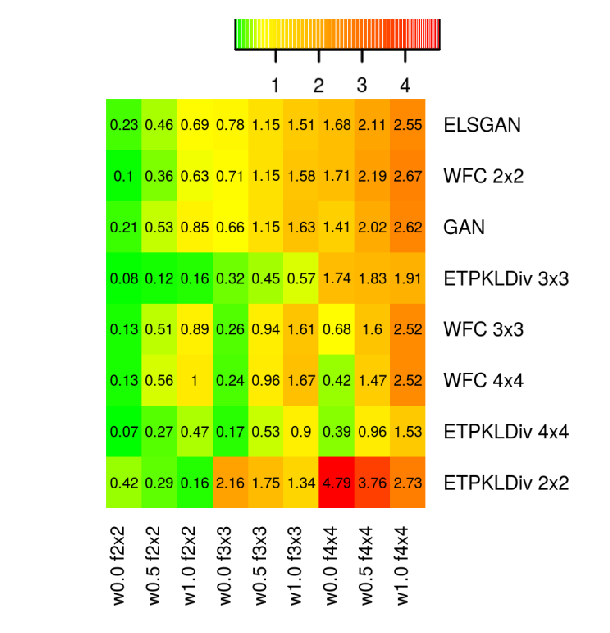
\includegraphics[width=0.5\textwidth]{Figure3.eps}
\centering
\caption{ ~\textbf{The final result quality based on \(D_{KL} \) measurement.} This shows ETPKLDiv with 3*3 and 4*4 tile patterns has best results. This figure is  is available in the research paper~\cite{ref_lncs1} on page 171.} \label{Figure3}
\end{figure}

\section{SUGGESTION ON FUTURE WORK}
The similarity is really an important criterion for judging a "good" game level, however, it is not the only one. These are some important rules that need to be met at a game level. 
Considering the following example (see Fig.4 and Fig.5):
\begin{figure}[!htb]
   \begin{minipage}{0.48\textwidth}
     \centering
     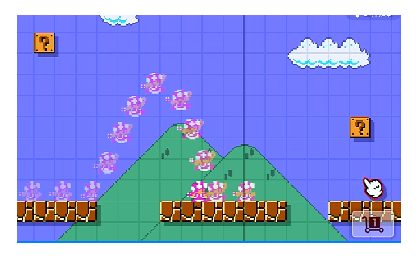
\includegraphics[width=.7\linewidth]{Figure4.eps}
     \caption{\textbf{Example of a passable level.} This level is made with game "Super Mario Maker 2".}\label{Figure4}
   \end{minipage}\hfill
   \begin{minipage}{0.48\textwidth}
     \centering
     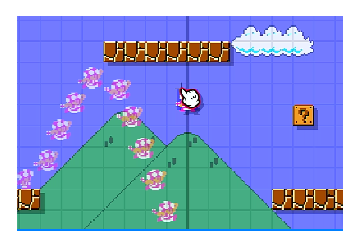
\includegraphics[width=.7\linewidth]{Figure5.eps}
     \caption{\textbf{Example of a impassable level.} This level is made with game "Super Mario Maker 2".}\label{Figure5}
   \end{minipage}
\end{figure}

Fig.4 is a passable level which means Mario can pass this level from the left to the right, while Fig.5 cannot. However, these two levels should have the same fitness based on the F(P, Q) (see section 3.3) measurement with up to 4*4 tile patterns generation. We can say Fig.4 is a "good" level, but not Fig.5 but F(P, Q) think they are equally "good".

One way to fix this is: add a process to check if it is passable. When doing this,(1) we can record the height of the left most platform as the current platform P(in Fig.4 and Fig.5, it is 2). (2)Ignore all the platforms 5 cells upper than the current platform (because Mario can just jump 5 cells higher), in Fig.5, the top-level platforms are ignored. (3)Look to the right, ignore all the platforms beyond the accessible range from the right edge of P. The relation of the right distance and difference in height shown in Table 2. (4) If there is no platform in the range -> not passable; Else: if the platform reaches the right of the level -> passable, else set the next platform as P and repeat process (2) to (4).

\begin{table}[h!]
\centering
\begin{tabular}{|c| c|} 
 \hline
 Height Above & Right Distance \\
 \hline
 within 2 & within 6  \\ 
 within 4 & within 5 \\
 within 5 & within 3 \\ [1ex] 
  \hline
\end{tabular}
\caption{\textbf{The relation of the right distance and difference in height}.}
\label{table2}
\end{table}

If the new level detected as "impassable", we use a \(\theta\)  within [0,1] to make \[F'(P,Q) = \theta \cdot F(P,Q)\].

Besides, there are some general rules, for example, the left part of the pipe should connect with the right part, the '?' block above the platform 6 cells are not reachable (see top left on Fig.4). These can also apply to \(\theta\).


\section{CONCLUSION AND FEEDBACK}
In conclusion, this article did well to design a fast, stable, and memory saving algorithm to make a good Super Mario Bros. game level, with limited training samples. The reprocessing of the formula of F(P, Q) (see section 3.3) and the Evolutionary Algorithm (see 3.4) chosen are extremely extraordinary. 

When reprocessing the formula of F(P, Q) from \(D_{KL}\) function to fit in with this challenge. The validation of P(X) and Q(x) avoid the risk of failure when training and the Symmetrical KL-Divergence approach increase the speed and Improved the results.

When choosing (1+1)EA as its Evolutionary Algorithm, they cleverly turn EA's weaknesses (cannot find a globally optimal solution) into strengths to make similar but not totally the same levels to the sample level.

Besides, using AI to make game level is a good try. The idea that converting making a "good" level to making a similar level as sample levels is helpful in my future study, but just consider the general rules in a game, for example, if the level is passable.

However, I doubt if the evaluation is fair enough. In other approaches, they just try to make a similar level, the value in \(D_{KL}\) become small is an indirect result, but in the ETPKLDiv, the decrease in \(D_{KL}\) is a direct result because that is a part of the fitness (see section 3.3). Note that this is only a guess, maybe in the future further work is needed to demonstrate its fairness.





\begin{thebibliography}{3}
\bibitem{ref_lncs1}
Simon M. Lucas and Vanessa Volz. 2019. Tile Pattern KL-Divergence for Analysing and Evolving Game Levels. In ~\textit{Genetic and Evolutionary Computation Conference (GECCO ’19), July 13–17, 2019, Prague, Czech Republic.}  ACM, New York, NY, USA, 9 pages.
 \doi{10.1145/3321707.3321781}
 

 
\bibitem{ref_article1}
Isaac Karth and Adam M. Smith. 2017. WaveFunction Collapse is Constraint Solving in the Wild.  ~\textit{International Conference on the Foundations of Digital Games (FDG)}.

\bibitem{ref_lncs2}
Vanessa Volz, Jacob Schrum, Jialin Liu, Simon M. Lucas, Adam M. Smith, and Sebastian Risi. 2018. Evolving Mario Levels in the Latent Space of a Deep Convolutional Generative Adversarial Network. In ~\textit{Proceedings of the Genetic and Evolutionary Computation Conference (GECCO 2018)}. ACM, New York, NY, USA, 8.  \doi{10.1145/3205455.3205517}





\end{thebibliography}
\end{document}
